\section{Research Plan} % or "Research Plan"
\label{sec:vis}

Our ultimate goal is to find a decent way to compare these multi-variate temporal data and design a visualization tool for civil engineers to interactively explore the whole dataset. We talk with our target users about what they need and summarize our visualization tasks as below:
\begin{itemize}
	\item [T1] An overview which summarizes all the earthquake simulations and can help them spotting weird ones
	\item [T2] For a specific earthquake simulation, there exists a context view to explore the multiviate dataset and help engineers  find interesting patterns 
	\item [T3] For the two views above, build efficient navigation and interaction between them 
\end{itemize} 


\subsection{Data Structure}
\label{sec:data}
\begin{figure}[h]
	\centering % avoid the use of \begin{center}...\end{center} and use \centering instead (more compact)
	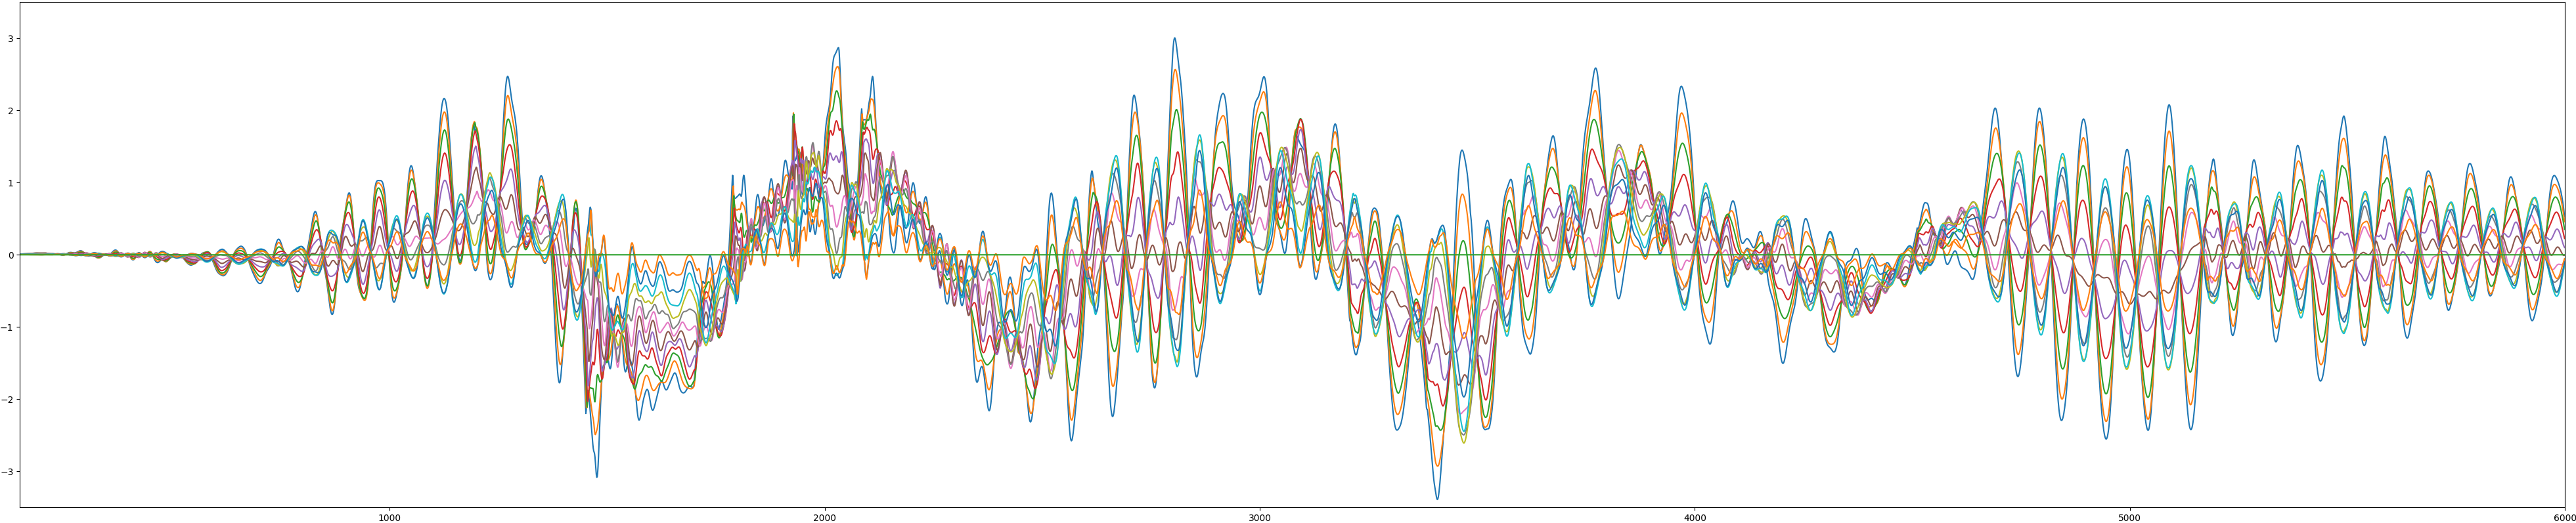
\includegraphics[width=\columnwidth]{figs/eq} 
	\caption{time series for "Shear" attribute of one earthquake simulation}
	\label{fig:data}
\end{figure}

Towards this end, we performed a pilot study using  earthquake simulation data generated by applying 50 different earthquakes to shake a 12-story building. The civil engineers calculated 6 attributes data which they considered most important: Acceleration/PGA, Shear, Diaphragm Force, Moment, Drift Ratio, Interstory Drift Ratio. For example,Shear is the stress component parallel to a given surface, such as a fault plane, that results from forces applied parallel to the surface or from remote forces transmitted through the surrounding rock. For each attribute, there are 13 time series data corresponding to 12 stories plus the ground. Then all the data are normalized and centered. Fig. 3 is one earthquake's Shear simulation time series for 13 stories which represented by 13 different colors. Fig. 4 is the structure of the whole dataset. Currently, in terms of comparing different simulation data, we have not extended to the cubic  which attribute dimension is added into.
\begin{figure}[h]
	\centering % avoid the use of \begin{center}...\end{center} and use \centering instead (more compact)
	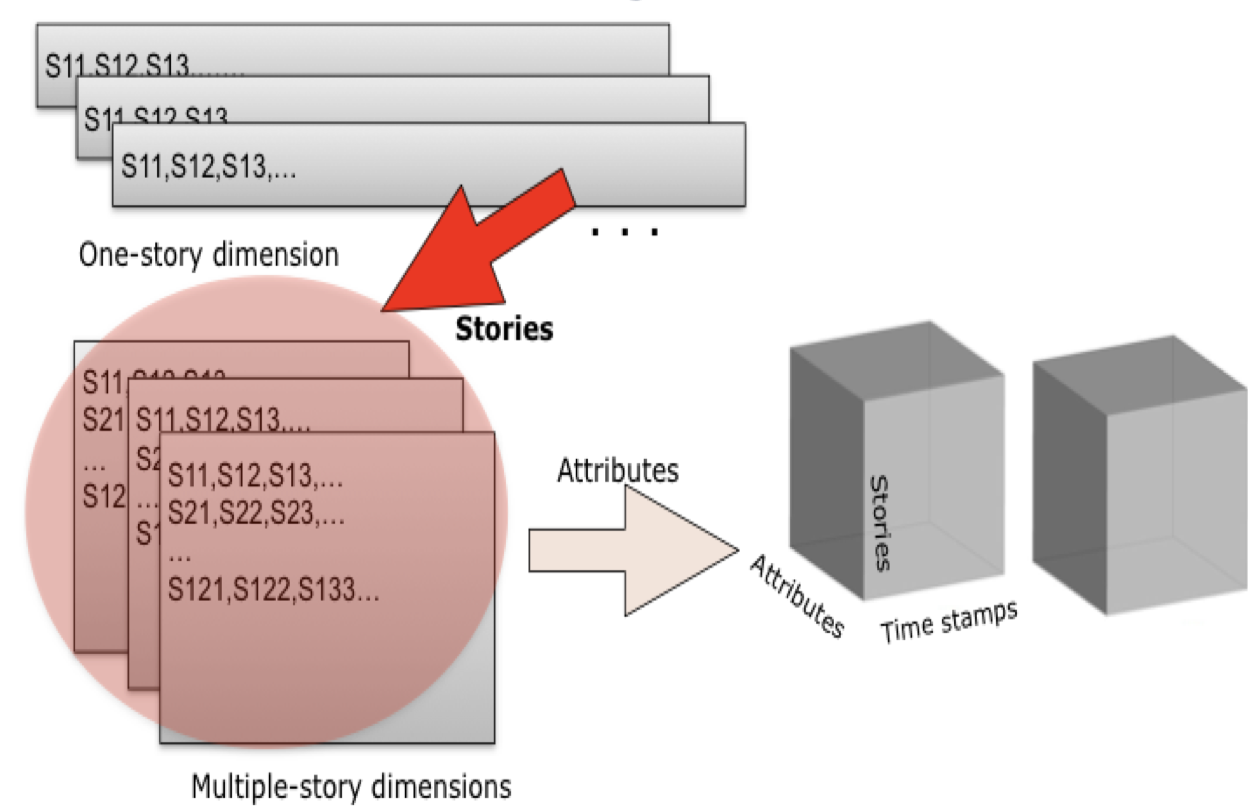
\includegraphics[width=\columnwidth]{figs/structure} 
	\caption{The overall structure of the earthquake simulations, the shading part is what we are working on right now}
	\label{fig:data}
\end{figure}


\subsection{Detailed Data View}
\label{sec:context }
This visualization view(Fig. 2) give users a way to explore one cubic database. It includes three parts: two time series plots for accerlation data, A heatmap plot for the time series of the other attributes and a 2D histogram to demonstrate the data value distribute of two selected attribute. The accerlation is the atrribute of the earthquake itself which will be same for all the stories at the same time stamps. We list it individually and these two plots obeying overview + details on demand which allows you to zoom and brush any  time intervals. In the heatmap, you can see the heatmap one attribute of this earthquake simulation data, you can navigate among different attributes and colormaps. The 2D histogram allow you to compare the the selected attribute in part B and any other attribute. Some interactions are built between between differrent parts which allow you to discover rare patterns and models.

\subsection{Overview View}
\label{sec:context }

\subsubsection{NLP Model and Probability Product Kernel}
\label{method}
The other view (Fig. 1) organize the whole dataset under a much more abstract way. Now we want to compare the Shear value among different earthquake data. Based on the fact and observation that earthquakes data has some repeated periods (Fig. 2).  We applied a big-of-words model to cut each earthquake simulation into a set of segments with a fixed period(P), the P is found using cross-correlation within itself. Each segment is a 13XP matrix.After applying the chopping method, each earthquake simulation becomes a set of matrices(motifs). For any two motifs coming from any two earthquakes, we could always calcuate the cosine similarity if we upsample one motif to the same length of the other. Eventually we could calculate the similarity of any two earthquake simulations with the same attribute. In order to capture more features and solving the problem that cross-correlation is not a kernel which may hurt the futher classification. we implicitly map these segments to a Hilbert Space and fit a Gaussian distribution to each earthquake simulation using Kernel PCA.~\cite{conf/icml/KondorJ03} Then we measure the similarity between earthquake simulations as Bhattacharyya’s measure of affinity between such Gaussians.
%TODO: add formula
\subsubsection{Matrix view}
\label{matrixvis}

The Adjacency Matrix view enables users to grasp a global view of one attribute among the all simulation data. We use D3 library which contains the existing adjacency matrix template~\cite{Bostock:2011:DDD:2068462.2068631}. Each grid in the matrix represents the similarity between two simulation data on this attribute.  We build a mouse over in this view, when the users move their mouse on the grid, the column and the row associated with that gird chosen will be highlighted with a bold border which will make it easier to obverse the column and the row. The view also consists a zoomable and navigation feature which can be used to filter the uninterested data based on the demand. Click on one of the grid will give another matrix comparing all the motifs from one earthquake simulation with all the motifs from the other.Theses two views allow users to explore interesting finding. For example, in Fig. 1, the first earthquake is similar to most of the others, the fifteenth, however, is quite different from the others. Clicking any of the label of the earthquake will also allow you navigate to the context view to further study the earthquake simulation you identify.


\
%\begin{figure*}[h]
% \centering 
% 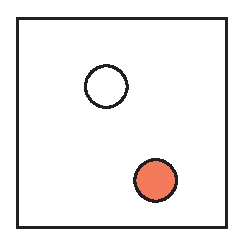
\includegraphics[width=\textwidth]{figs/sample} 
% \caption{Double Column Figure.}
% \label{fig:sample2}
%\end{figure*}

